\clearpage

\lehead[]{\sf\hspace*{-2.00cm}\textcolor{white}{\colorbox{lightblue}{\parbox[c][0.70cm][b]{1.60cm}{
\makebox[1.60cm][r]{\thechapter}\\ \makebox[1.60cm][r]{ÜBUNG}}}}\hspace{0.17cm}\textcolor{lightblue}{\chaptertitle}}
\rohead[]{\textcolor{lightblue}{\chaptertitle}\sf\hspace*{0.17cm}\textcolor{white}{\colorbox{lightblue}{\parbox[c][0.70cm][b]{1.60cm}{\thechapter\\
ÜBUNG}}}\hspace{-2.00cm}}
%\chead[]{}
\rehead[]{\textcolor{lightblue}{AvHG, Inf, My}}
\lohead[]{\textcolor{lightblue}{AvHG, Inf, My}}

\section{Dateizugriffe -- Übungen}

\subsection{Aufgabe 1: Zeichen zählen}

Schreibe ein Programm, das zählt, wie viele Kleinbuchstaben, Großbuchstaben,
Ziffern, Trennzeichen und sonstige Zeichen in einer Datei stehen. Das Ergebnis
soll in einer \myClass{JList}-Komponente ausgegeben werden.

Beachte, dass die \myClass{JList}-Komponente vor der Auswertung einer Datei
gelöscht werden muss, um eventuell vorhandene alte Inhalte zu entfernen. Gib in einer
Messagebox eine Fehlermeldung aus, falls die angegebene Datei nicht existiert.

\begin{center}
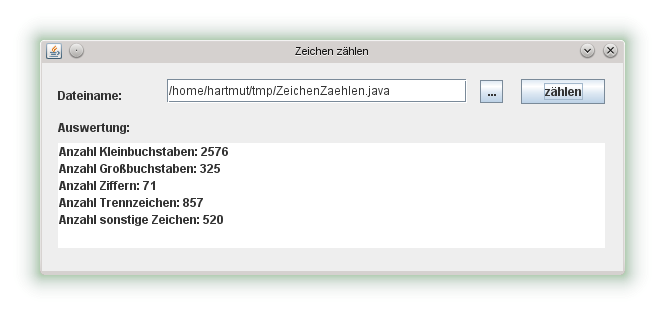
\includegraphics[width=0.85\textwidth]{./inf/SEKII/27_Java_Dateizugriffe/ZeichenZaehlen.png}
\end{center}

Verwende zum Zählen der verschiedenen Arten von Zeichen die folgenden Methoden
der Klasse \myClass{Character} (siehe Online-Hilfe):

\bgroup
\def\arraystretch{1.2}
\begin{tabularx}{\textwidth}{|p{70mm}|X|}
\hline
\textbf{Methode} & \textbf{Erläuterung}
\\ \hline
\lstinline|static boolean isDigit(char ch)| & 
Prüft, ob der angegebene Buchstabe eine Ziffer (0 bis 9) ist.
\\ \hline
\lstinline|static boolean isLowerCase(char ch)| &
Prüft, ob das angegebene Zeichen ein Kleinbuchstabe ist. 
\\ \hline
\lstinline|static boolean isUpperCase(char ch)| &
Prüft, ob das angegebene Zeichen ein Großbuchstabe ist. 
\\ \hline
\lstinline|static boolean isWhitespace(char ch)| &
Prüft, ob der angegebene Buchstabe ein Trennzeichen ist (Leerzeichen,
Tabulator, Zeilenumbruch, usw.) \\ \hline
\end{tabularx}
\egroup

\subsubsection{Zusatzaufgabe}

Zum Laden einer Datei bietet Java die Klasse \myClass{JFileChooser} an. Wenn man
ein Objekt dieser Klasse erstellt, erscheint der Standarddialog zum Suchen nach
einer Datei. Informiere dich in der Online-Hilfe darüber, wie man die Klasse
\myClass{JFileChooser} benutzt, und baue sie in dein Programm ein. Rechts neben
dem Textfeld für den Dateinamen sollte ein Button mit der Aufschrift
\glqq ...\grqq\ eingefügt werden. Wenn der Benutzer auf den Button klickt,
erscheint der Dialog zum Suchen nach einer Datei. Der Dateiname wird nach dem
Schließen des Dialogs in das Textfeld eingetragen.


\subsection{Aufgabe 2: Einfache Verschlüsselung mit dem Caesar-Verfahren}

Die sogenannte  Caesar-Verschlüsselung ist schon über 2000 Jahre alt wurde von
Julius Caesar 50 Jahre vor Christus benutzt. Das Alphabet wird dabei einfach um
mehrere Buchstaben verschoben. Zum Beispiel um drei Buchstaben:

ABC\textbf{DEFGHIJKLMNOPQRSTUVWXYZ}

\textbf{DEFGHIJKLMNOPQRSTUVWXYZ}ABC

Damit wird aus dem Klartext \myUserInput{hallo} der Geheimtext
\myUserInput{KDOOR}.

\begin{compactenum}[a)]
\item Erstelle ein Programm, das den Inhalt einer Datei einliest und mit dem
Caesar-Verfahren verschlüsselt in eine zweite Datei schreibt. Verschlüsselt
werden sollen nur Buchstaben von \myUserInput{a} bis \myUserInput{z}. Alle
anderen Zeichen sollen unverändert bleiben. Wandle zu Beginn alle Buchstaben in
der Datei mit der Methode \lstinline|Character.toLowerCase()| in
Kleinbuchstaben um (siehe Online-Hilfe).

\begin{minipage}{0.35\textwidth}
Anmerkung:

Mit Variablen vom Typ \lstinline|char| kann man wie mit Zahlen rechnen.

Beispiel:

\begin{lstlisting}
char c = 'b';
if (c >= 'a' && c <= 'z') {
    c = (char) (c + 3);
}
int differenz = c - 'a';
\end{lstlisting}

\end{minipage}
\begin{minipage}{0.65\textwidth}
\begin{center}
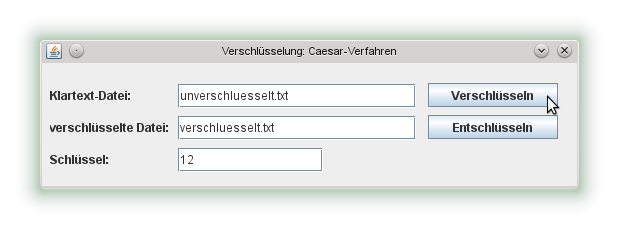
\includegraphics[width=0.9\textwidth]{./inf/SEKII/27_Java_Dateizugriffe/Verschluesselung.png}
\end{center}
\end{minipage}

\item Erweitere das Programm so, dass der Inhalt einer verschlüsselten Datei
auch wieder entschlüsseln werden kann. Der Inhalt der Eingabedatei soll wie im
ersten Aufgabenteil in eine Ausgabedatei geschrieben werden, nur diesmal nicht
\emph{ver}schlüsselt sondern \emph{ent}schlüsselt.
\end{compactenum}


\subsection{Aufgabe 3: Prüfsumme}

Um Sicherzustellen, dass der Inhalt einer Datei nicht manipuliert wurde,
berechnet man häufig eine sogenannte \emph{Prüfsumme}. Die Prüfsumme ist eine
Zahl, die entsteht, wenn man alle Bytes der Datei miteinander verknüpft. Das
einfachste Verfahren zur Berechnung einer Prüfsumme funktioniert
folgendermaßen:

Es wird ein Byte für die Prüfsumme angelegt, das zu Beginn den Wert Null
enthält. Alle Bytes, die in der Datei enthalten sind, werden der Reihe nach mit
dem Prüf-Byte mit einer Exklusiv-ODER Verknüpfung verbunden. Java-Beispiel:

\begin{lstlisting}
checksum = (byte) (checksum ^ b1);
\end{lstlisting}

Die Exklusiv-ODER Verknüpfung verknüpft die einander entsprechenden Bits der
beiden Bytes. Das Ergebnis-Bit ist immer dann wahr (1), wenn beide Bits
ungleich sind, und falsch (0), wenn beide Bits gleich sind.

Es soll nach dem oben beschriebenen Verfahren für eine Datei eine Prüfsumme
generiert werden, damit überprüft werden kann, ob der Datei-Inhalt manipuliert
wurde.

\begin{compactenum}[a)]
\item Wenn man auf den linken Button drückt, soll für eine Datei eine Prüfsumme
generiert werden. Es wird aus der Eingabedatei eine /home/hartmut/tmpneue Datei
generiert, die um die Prüfsumme erweitert ist. Das Ergebnis wird unter dem Namen der
Ausgabedatei abgespeichert. Falls die Eingabedatei nicht existiert wird in
einer Messagebox eine Fehlermeldung ausgegeben.

In die Ausgabedatei wird als erstes Zeichen ein \lstinline|$| geschrieben, um
zu markieren, dass diese Datei eine Prüfsumme enthält. Dann folgt der
eigentliche Inhalt der Datei, und als letztes Byte wird die generierte
Prüfsumme angehängt.

\item Wenn man auf den rechten Button drückt, wird geprüft, ob die Prüfsumme der
Eingabedatei korrekt ist oder ob der Inhalt der Datei verändert wurde. Falls
die Datei am Anfang kein \lstinline|$| enthält, besitzt sie keine Prüfsumme,
und es wird in einer Messagebox eine Fehlermeldung ausgegeben. Es wird ebenso
eine Fehlermeldung ausgegeben, falls die Eingabedatei nicht existiert.

Wenn eine Prüfsumme vorhanden ist, wird die Prüfsumme über den Inhalt der Datei
(ohne das voran gehängte \lstinline|$| und das Prüfbit am Ende) erneut
berechnet und mit dem letzten Byte verglichen. Sind beide Werte gleich, wird
dem Benutzer in einer Messagebox mitgeteilt, dass der Datei-Inhalt nicht
verfälscht wurde. Falls die Werte ungleich sind, erhält der Benutzer die
Mitteilung, dass die Datei manipuliert wurde.

\begin{center}
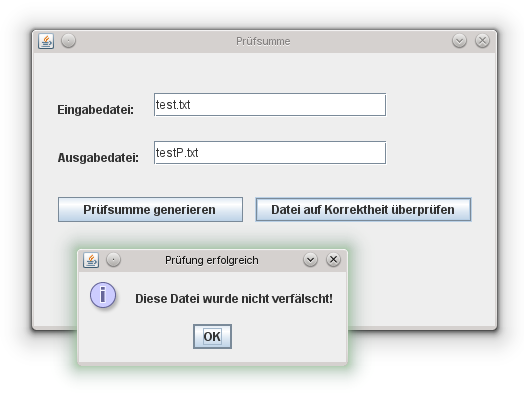
\includegraphics[width=0.6\textwidth]{./inf/SEKII/27_Java_Dateizugriffe/Pruefsumme.png}
\end{center}

Du kannst es mit einer beliebigen Datei selbst austesten: Dieses einfache
Prüfsummenverfahren funktioniert! Sobald man in der Datei ein oder mehrere
Zeichen verändert, kommt mit hoher Sicherheit eine andere Prüfsumme heraus.
\end{compactenum}


\subsection{Aufgabe 4: Notizbuch}

\begin{compactenum}
\item Erstelle die folgende Programmoberfläche: 

\begin{center}
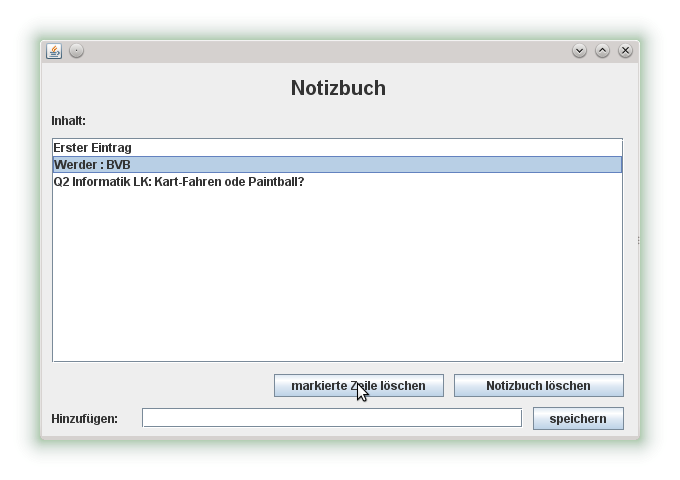
\includegraphics[width=0.8\textwidth]{./inf/SEKII/27_Java_Dateizugriffe/Notizbuch.png}
\end{center}

Die obere Komponente mit der
Beschriftung \glqq Inhalt:\grqq\ soll eine \myClass{JList} sein (keine
\myClass{JTextArea}).

\item Der Benutzer kann in das JTextField neue Einträge für das Notizbuch
eingeben. Wenn er auf den \glqq speichern\grqq -Button drückt, liest das
Programm den Text aus dem Textfeld aus und hängt ein \lstinline|$| an das
String-Ende an. Anschließend öffnet es eine Datei mit dem Namen
\myFile{notizen.txt} zum Schreiben und schreibt den neuen Eintrag in die Datei.
Falls die Datei bereits existiert, soll der neue Text an den vorhandenen Text
angehängt werden. Dies geschieht automatisch, wenn du beim Erzeugen des
\myClass{FileOutputStream}-Objektes den Wert \lstinline|true| als zweiten
Parameter übergibst.

Beispiel:

\begin{lstlisting}
FileOutputStream fileOut = new FileOutputStream("notizen.txt", true);
\end{lstlisting}

\item Nach dem Abspeichern eines neuen Eintrags und ebenso beim Neustart der
Datei, soll der aktuelle Inhalt der Datei \myFile{notizen.txt} in die
\myClass{JList}-Komponente geschrieben werden. Lösche dazu zunächst den Inhalt
der Listkomponente (für den Fall, dass sich noch alte Daten in der Komponente
befinden) und lies dann den Inhalt der Datei ein. Ein \lstinline|$| markiert
jeweils das Ende einer Zeile, das heißt wenn du ein \lstinline|$|-Zeichen liest,
solltest du alle seit dem letzten \lstinline|$|-Zeichen eingelesenen Buchstaben
mit \lstinline|addElement()| in das  \myClass{DefaultListModel}-Objekt der
\myClass{JList}-Komponente einfügen.

\item Wenn man auf den Button \glqq Notizbuch löschen\grqq\ klickt, soll der
Inhalt der Datei gelöscht werden. Anschließend wird die
\myClass{JList}-Komponente aktualisiert. Die Datei kannst du sehr einfach
löschen, in dem du ein neues \myClass{FileOutputStream}-Objekt anlegst, und es
wieder schließt ohne etwas hinein zu schreiben. Beachte, dass dieses Mal beim
Anlegen des Objektes als zweiter Parameter der Wert \lstinline|false| übergeben
werden muss (dies bedeutet, dass der neue Inhalt nicht an den vorhandenen
Inhalt angehängt wird).

\item Wenn der Benutzer auf den Button \glqq markierte Zeile löschen\grqq\
klickt, soll die markierte Zeile aus der \myClass{JList}-Komponente gelöscht
werden. Anschließend wird der verbleibende Inhalt der List-Komponente in die
Datei \myFile{notizen.txt} geschrieben. Zum Löschen des markierten Eintrags aus
der \myClass{JList}-Komponente liest du zunächst mit
\lstinline|getSelectedIndex()| (eine Methode des
\myClass{DefaultListModel}-Objektes) den markierten Eintrag aus. Falls keine
Zeile markiert ist, wird mit einer Fehlermeldung abgebrochen. Andernfalls rufst
du anschließend die folgende Methode der List-Komponente auf:

\begin{lstlisting}
public void remove(int index)
\end{lstlisting}

Dies ist ebenfalls eine Methode des  \myClass{DefaultListModel}-Objektes.
Danach ist die List-Komponente verändert und du musst den Inhalt der
\myClass{JList}-Komponente zeilenweise auslesen und in die Datei schreiben.
Beachte, dass du beim Anlegen des \myClass{FileOutputStream}-Objektes wie bei
Teilaufgabe d) den Wert \lstinline|false| als zweiten Parameter übergeben musst,
damit die vorhandene Datei überschrieben wird. Die Methode \lstinline|getSize()|
des \myClass{DefaultListModel}-Objektes liefert die Anzahl der Zeilen zurück.
Gehe alle Zeilen in einer Schleife durch. Mit der folgenden Methode kannst du
dir den Text in einer Zeile mit einer bestimmten Nummer holen (die
Zeilennummerierung beginnt mit 0):

\begin{lstlisting}
public String get(int index)
\end{lstlisting}

Beachte, dass du vor dem Schreiben einer Zeile in die Datei noch ein
\lstinline|$| an den Text anhängen musst.
\end{compactenum}
